\ifdefined\included
\else
\documentclass[a4paper,11pt,twoside]{StyleThese}
\usepackage{amsmath,amssymb, amsthm}             % AMS Math
\usepackage[T1]{fontenc}
\usepackage[utf8x]{inputenc}
\usepackage{babel}
\usepackage{datetime}

\usepackage{silence}

\WarningFilter{minitoc(hints)}{W0023}
\WarningFilter{minitoc(hints)}{W0028}
\WarningFilter{minitoc(hints)}{W0030}

\usepackage{lmodern}
\usepackage{tabularx}
%\usepackage{tabular}
\usepackage{multirow}
\usepackage{xspace}

\usepackage{subfig}
\usepackage[inline]{enumitem}

\usepackage{hhline}
\usepackage[left=1.5in,right=1.3in,top=1.1in,bottom=1.1in,includefoot,includehead,headheight=13.6pt]{geometry}
\renewcommand{\baselinestretch}{1.05}

% Table of contents for each chapter

\usepackage[nottoc, notlof, notlot]{tocbibind}
\usepackage{minitoc}
\setcounter{minitocdepth}{2}
\mtcindent=15pt
% Use \minitoc where to put a table of contents

\usepackage{aecompl}

% Glossary / list of abbreviations

\usepackage[intoc]{nomencl}
\iftoggle{ThesisInEnglish}{%
\renewcommand{\nomname}{Glossary}
}{ %
\renewcommand{\nomname}{Liste des Abréviations}
}

\usepackage{etoolbox}
\renewcommand\nomgroup[1]{%
  \item[\bfseries
  \ifstrequal{#1}{A}{Number Sets}{%
  \ifstrequal{#1}{G}{Agents Beliefs and Action Models}{%
  \ifstrequal{#1}{N}{Navigation}{%
  \ifstrequal{#1}{O}{Ontology}{%
  \ifstrequal{#1}{R}{Referring Expression Generation}{%
  \ifstrequal{#1}{Z}{Controllable and Uncontrollable Agents Task Planning}{}}}}}}%
]}

\makenomenclature



% My pdf code

\usepackage{ifpdf}

\ifpdf
  \usepackage[pdftex]{graphicx}
  \DeclareGraphicsExtensions{.jpg}
  \usepackage[pagebackref,hyperindex=true]{hyperref}
  \usepackage{tikz}
  \usetikzlibrary{arrows,shapes,calc}
\else
  \usepackage{graphicx}
  \DeclareGraphicsExtensions{.ps,.eps}
  \usepackage[dvipdfm,pagebackref,hyperindex=true]{hyperref}
\fi

\graphicspath{{.}{images/}}

%% nicer backref links. NOTE: The flag ThesisInEnglish is used to define the
% language in the back references. Read more about it in These.tex

\iftoggle{ThesisInEnglish}{%
\renewcommand*{\backref}[1]{}
\renewcommand*{\backrefalt}[4]{%
\ifcase #1 %
(Not cited.)%
\or
(Cited in page~#2.)%
\else
(Cited in pages~#2.)%
\fi}
\renewcommand*{\backrefsep}{, }
\renewcommand*{\backreftwosep}{ and~}
\renewcommand*{\backreflastsep}{ and~}
}{%
\renewcommand*{\backref}[1]{}
\renewcommand*{\backrefalt}[4]{%
\ifcase #1 %
(Non cité.)%
\or
(Cité en page~#2.)%
\else
(Cité en pages~#2.)%
\fi}
\renewcommand*{\backrefsep}{, }
\renewcommand*{\backreftwosep}{ et~}
\renewcommand*{\backreflastsep}{ et~}
}

% Links in pdf
\usepackage{color}
\definecolor{linkcol}{rgb}{0,0,0.4} 
\definecolor{citecol}{rgb}{0.5,0,0} 
\definecolor{linkcol}{rgb}{0,0,0} 
\definecolor{citecol}{rgb}{0,0,0}
% Change this to change the informations included in the pdf file

\hypersetup
{
bookmarksopen=true,
pdftitle="Endowing the robot with the abilities to control and evaluate its contribution to a human-robot joint action",
pdfauthor="Amandine MAYIMA", %auteur du document
pdfsubject="Thèse", %sujet du document
%pdftoolbar=false, %barre d'outils non visible
pdfmenubar=true, %barre de menu visible
pdfhighlight=/O, %effet d'un clic sur un lien hypertexte
colorlinks=true, %couleurs sur les liens hypertextes
pdfpagemode=None, %aucun mode de page
pdfpagelayout=SinglePage, %ouverture en simple page
pdffitwindow=true, %pages ouvertes entierement dans toute la fenetre
linkcolor=linkcol, %couleur des liens hypertextes internes
citecolor=citecol, %couleur des liens pour les citations
urlcolor=linkcol %couleur des liens pour les url
}

% definitions.
% -------------------

\setcounter{secnumdepth}{3}
\setcounter{tocdepth}{2}

% Some useful commands and shortcut for maths:  partial derivative and stuff

\newcommand{\pd}[2]{\frac{\partial #1}{\partial #2}}
\def\abs{\operatorname{abs}}
\def\argmax{\operatornamewithlimits{arg\,max}}
\def\argmin{\operatornamewithlimits{arg\,min}}
\def\diag{\operatorname{Diag}}
\newcommand{\eqRef}[1]{(\ref{#1})}

\usepackage{rotating}                    % Sideways of figures & tables
%\usepackage{bibunits}
%\usepackage[sectionbib]{chapterbib}          % Cross-reference package (Natural BiB)
%\usepackage{natbib}                  % Put References at the end of each chapter
                                         % Do not put 'sectionbib' option here.
                                         % Sectionbib option in 'natbib' will do.
\usepackage{fancyhdr}                    % Fancy Header and Footer

% \usepackage{txfonts}                     % Public Times New Roman text & math font
  
%%% Fancy Header %%%%%%%%%%%%%%%%%%%%%%%%%%%%%%%%%%%%%%%%%%%%%%%%%%%%%%%%%%%%%%%%%%
% Fancy Header Style Options

\pagestyle{fancy}                       % Sets fancy header and footer
\fancyfoot{}                            % Delete current footer settings

%\renewcommand{\chaptermark}[1]{         % Lower Case Chapter marker style
%  \markboth{\chaptername\ \thechapter.\ #1}}{}} %

%\renewcommand{\sectionmark}[1]{         % Lower case Section marker style
%  \markright{\thesection.\ #1}}         %

\fancyhead[LE,RO]{\bfseries\thepage}    % Page number (boldface) in left on even
% pages and right on odd pages
\fancyhead[RE]{\bfseries\nouppercase{\leftmark}}      % Chapter in the right on even pages
\fancyhead[LO]{\bfseries\nouppercase{\rightmark}}     % Section in the left on odd pages

\let\headruleORIG\headrule
\renewcommand{\headrule}{\color{black} \headruleORIG}
\renewcommand{\headrulewidth}{1.0pt}
\usepackage{colortbl}
\arrayrulecolor{black}

\fancypagestyle{plain}{
  \fancyhead{}
  \fancyfoot{}
  \renewcommand{\headrulewidth}{0pt}
}

%\usepackage{MyAlgorithm}
%\usepackage[noend]{MyAlgorithmic}
\usepackage{algorithm}
\usepackage[noend]{algpseudocode}
\usepackage{comment}
\usepackage[ED=MITT-InfoTel, Ets=INSA]{tlsflyleaf}
%%% Clear Header %%%%%%%%%%%%%%%%%%%%%%%%%%%%%%%%%%%%%%%%%%%%%%%%%%%%%%%%%%%%%%%%%%
% Clear Header Style on the Last Empty Odd pages
\makeatletter

\def\cleardoublepage{\clearpage\if@twoside \ifodd\c@page\else%
  \hbox{}%
  \thispagestyle{empty}%              % Empty header styles
  \newpage%
  \if@twocolumn\hbox{}\newpage\fi\fi\fi}

\newcommand*{\algrule}[1][\algorithmicindent]{%
	\makebox[#1][l]{%
		\hspace*{.2em}% <------------- This is where the rule starts from
		\vrule height .75\baselineskip depth .25\baselineskip
	}
}

%%% to have lines in algorithm, from stackexchange
\newcount\ALG@printindent@tempcnta
\def\ALG@printindent{%
	\ifnum \theALG@nested>0% is there anything to print
	\ifx\ALG@text\ALG@x@notext% is this an end group without any text?
	% do nothing
	\else
	\unskip
	% draw a rule for each indent level
	\ALG@printindent@tempcnta=1
	\loop
	\algrule[\csname ALG@ind@\the\ALG@printindent@tempcnta\endcsname]%
	\advance \ALG@printindent@tempcnta 1
	\ifnum \ALG@printindent@tempcnta<\numexpr\theALG@nested+1\relax
	\repeat
	\fi
	\fi
}
% the following line injects our new indent handling code in place of the default spacing
\patchcmd{\ALG@doentity}{\noindent\hskip\ALG@tlm}{\ALG@printindent}{}{\errmessage{failed to patch}}
\patchcmd{\ALG@doentity}{\item[]\nointerlineskip}{}{}{} % no spurious vertical space
% end vertical rule patch for algorithmicx

\makeatother
 
%%%%%%%%%%%%%%%%%%%%%%%%%%%%%%%%%%%%%%%%%%%%%%%%%%%%%%%%%%%%%%%%%%%%%%%%%%%%%%% 
% Prints your review date and 'Draft Version' (From Josullvn, CS, CMU)
\newcommand{\reviewtimetoday}[2]{\special{!userdict begin
    /bop-hook{gsave 20 710 translate 45 rotate 0.8 setgray
      /Times-Roman findfont 12 scalefont setfont 0 0   moveto (#1) show
      0 -12 moveto (#2) show grestore}def end}}
% You can turn on or off this option.
% \reviewtimetoday{\today}{Draft Version}
%%%%%%%%%%%%%%%%%%%%%%%%%%%%%%%%%%%%%%%%%%%%%%%%%%%%%%%%%%%%%%%%%%%%%%%%%%%%%%% 

\newenvironment{maxime}[1]
{
\vspace*{0cm}
\hfill
\begin{minipage}{0.5\textwidth}%
%\rule[0.5ex]{\textwidth}{0.1mm}\\%
\hrulefill $\:$ {\bf #1}\\
%\vspace*{-0.25cm}
\it 
}%
{%

\hrulefill
\vspace*{0.5cm}%
\end{minipage}
}

\let\minitocORIG\minitoc
\renewcommand{\minitoc}{\minitocORIG \vspace{1.5em}}

\usepackage{multirow}
%\usepackage{slashbox}

\newenvironment{bulletList}%
{ \begin{list}%
	{\tiny$\bullet$}%
	{\setlength{\labelwidth}{25pt}%
	 \setlength{\leftmargin}{30pt}%
	 \setlength{\itemsep}{-0.5em}}}%
{ \end{list} }

\newenvironment{inlineEnumerate}
{\begin{enumerate*} [label={(\arabic*)}] }
{\end{enumerate*}}

\theoremstyle{definition}
\newtheorem{definition}{Definition}
\renewcommand{\epsilon}{\varepsilon}

% centered page environment

\newenvironment{vcenterpage}
{\newpage\vspace*{\fill}\thispagestyle{empty}\renewcommand{\headrulewidth}{0pt}}
{\vspace*{\fill}}

\newenvironment{asl}{\ttfamily\begin{tabbing}~~~\=$\leftarrow$ \= ~~~ \=
		\kill}{\end{tabbing}}

\usepackage{tablefootnote}

\theoremstyle{plain}
\newtheorem{constraint}{Constraint}[section]

\algnewcommand\algorithmicforeach{\textbf{for each}}
\algnewcommand\algorithmicin{\textbf{in}}
\algdef{S}[FOR]{ForEach}[2]{\algorithmicforeach\ #1\ \algorithmicin\ #2\ \algorithmicdo}

\algnewcommand\algorithmicforkxor{\textbf{do fork-join-xor}}
\algnewcommand\algorithmicendforkxor{\textbf{end fork-join-xor}}
\algdef{SE}{ForkXor}{EndForkXor}{\algorithmicforkxor}{\algorithmicendforkxor}


\usepackage{listings}
\lstset{
	frame=single,
	captionpos=b,
	breaklines=true,
	basicstyle=\ttfamily,
	numberstyle=\color{black},
	tabsize=2,
	mathescape=true,
	literate=%
		{â}{{\^a}}1
}

\lstdefinestyle{inline}{
	frame=none,
	aboveskip=\smallskipamount,
	belowskip=\smallskipamount,
}

\lstdefinestyle{OwlTurtle}{
	language=C,
	tabsize=4,
	basicstyle=\scriptsize\ttfamily,
	keywordstyle=\bfseries\color{darkgray},
	morekeywords={rdf:type, rdfs:domain, rdfs:subPropertyOf, rdfs:range, :hasSubtask, :DecompositionUsedBy, rdfs:subClassOf, :hasDecomposition, owl:inverseOf, htn_actions:hasEffect, rdfs:label},
	alsoletter=:
}

\lstdefinestyle{aslDef}{
	frame=none,
%	breaklines=false,
	%xleftmargin=.1\textwidth, xrightmargin=.1\textwidth
}

\fancypagestyle{example}{%
	\fancyhead[LE]{\bfseries\thepage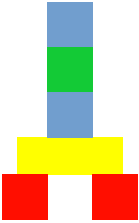
\includegraphics[scale=0.20]{figures/chapter2/task_goal.pdf}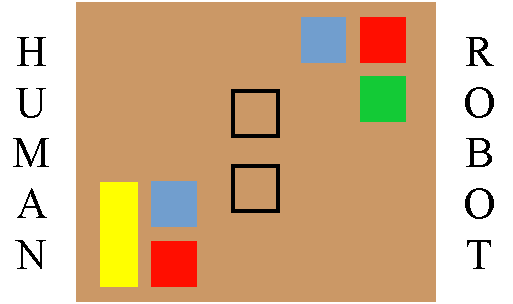
\includegraphics[scale=0.18]{figures/chapter2/task_setup_mini.pdf}}   
	\fancyhead[RO]{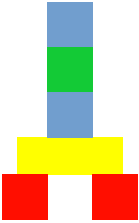
\includegraphics[scale=0.20]{figures/chapter2/task_goal.pdf}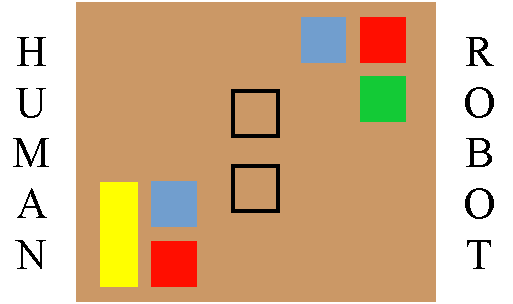
\includegraphics[scale=0.18]{figures/chapter2/task_setup_mini.pdf}\bfseries\thepage}  
	\fancyhead[RE]{\bfseries\nouppercase{\leftmark}}      % Chapter in the right on even pages
	\fancyhead[LO]{\bfseries\nouppercase{\rightmark}}     % Section in the left on odd pages
}%

\usepackage{pdfpages}
\usepackage{makecell}
\usepackage{pdflscape} 
\usepackage{mathtools}
\usepackage[section]{placeins}
\usepackage{afterpage}

%%%%%%%% my commands
\newcommand{\etal}{\textit{et al}.}
\newcommand{\ie}{\textit{i.e.}, }
\newcommand{\eg}{\textit{e.g.}, }
\newcommand{\fact}[3]{\mbox{\textit{#1}(#2, #3)}}
\newcommand{\circledtext}[1]{\raisebox{.5pt}{\textcircled{\raisebox{-.9pt} {#1}}}}
\newcommand{\sparql}{\textsc{SPARQL}}

\newcommand{\algConst}[1]{${\scriptscriptstyle #1}$}
\newcommand{\algNormTextSub}[2]{$\text{#1}_{#2}$}

\newcommand{\aslnumber}[1]{$#1$}
\newcommand{\aslstring}[1]{\textsf{#1}}
\newcommand{\aslvar}[1]{\textcolor{purple}{\textit{#1}}}
\newcommand{\asllabel}[1]{\textbf{#1}}
\newcommand{\annotation}[1]{{\footnotesize #1}}
\newcommand{\rulebody}[1]{\mbox{\hspace{.05\linewidth}}\begin{minipage}[t]{0.9\linewidth}#1.\end{minipage}}
\newcommand{\context}[1]{\begin{minipage}[t]{0.9\linewidth}#1\end{minipage}}
\newcommand{\planbody}[1]{\begin{minipage}[t]{0.9\linewidth}#1.\end{minipage}}
\newcommand{\Jason}[0]{\textbf{\textit{Jason}}}
\newcommand{\sn}{\mbox{\large\textbf{\texttt{\textasciitilde}}}}


\sloppy
\begin{document}
\fi


\chapter*{Introduction}
\addstarredchapter{Introduction} %Sinon cela n'apparait pas dans la table des matières
\markboth{INTRODUCTION}{}

Robots will interact more and more with humans in the future and thus will need to be endowed with the pertinent abilities. We are still far from having autonomous robots among humans and able to smoothly collaborate with them.

A lot of research focus on abilities needed to the robot to make it more intelligent, useful and adaptive: the planning, the perception, the knowledge management, the navigation, the action recognition, the dialog... But those does not make a robot function, those does not make a robot collaborate with a human in a task. What does? The supervision. Indeed, this component, such a puppeteer, controls from above the wires of the other architecture components. Leaning on them, it makes the decisions about how and when the robot should act, in a collaborative task with a human, it decides what the robot should say; reacting to the environment, the human behavior and the human speech. A robot should be able to act following a plan but more importantly, it should be able to react to the unexpected or to (robotic or human) errors. And what can give a robot such abilities? A supervision component, or we should say, a component with a vision.

Thereby, given the central role of this component, we could thought that it is extensively studied in \acrlong{hri}, a field of research whose aims is to build robots that will autonomously interact with humans. However, it is not. This lack led to a slight change of subject for this thesis. Indeed, initially, the goal was to devise a supervisor making the robot robust to a number of contingencies that could happen during a human-robot interaction. But, in order to have a supervisor handling contingencies, we needed first a supervisor for ``non-contingent'' situations. Well, we could not find any existing system implementing a supervision component in the context of human-robot collaborative tasks, on which we could build contingencies handling. Thus, we devised it.

\section*{A Supervision for \acrlong{hri}}
\markright{A Supervision for \acrlong{hri}}
When humans collaborate to achieve a task together, numerous neurocognitive mechanisms come into play, more than we would have thought at first glance. Some of these mechanisms are also triggered in humans’ minds when they interact with robots as they are essential to a successful collaboration. Therefore, it is important for roboticists designing robots that will closely interact with humans to be aware of and take into account the humans mental states and sensori-motor functions involved in controlling and smoothing collaborative task performance. However, this does not imply that robots have to be endowed with the same mechanisms since being able to collaborate with humans does not mean to imitate them. What is key to roboticists is to understand how humans work and to design  robots that will adapt. Consequently, we closely collaborated with a psychologist and a philosopher in order to learn the keys of human collaboration such as joint action, commitment, shared representations...(Chapter~\ref{chapter:chap1}) It was also back and forth discussions between them and us, trying to close the gap between what abilities a robot should have and what is currently technically possible.

Thus, when designing and implementing our supervisor for human-robot collaborative tasks, our minds were well nourished. In this thesis, we tackled the issue of a real component supervision for \acrshort{hri}. It endows the robot with a number of abilities in order to make the robot the best partner possible for humans such as modeling their mental states or adapting to their decisions (Chapter~\ref{chapter:chap5} and Chapter~\ref{chapter:chap6}).

\section*{A first step toward contingency handling}
\markright{A first step toward contingency handling}

Even though we could not lean on an existing supervision system in order to endow a robot with abilities making it able to cope with the unexpected, we started brainstorming on the subject. We realized that before being able to handle with contingencies, the robot should be able notice them. But, is it necessary to react immediately when something derails a bit or should there be a kind of threshold? As humans, sometimes, we run into minor incidents when performing a task for example, but as the situation is good overall, we tolerate it. Thus, we came with a novel idea: to give the robot the ability to evaluate, in real-time, the quality of its interaction with its human partner (Chapter~\ref{chapter:chap7}). This is a first step toward contingency handling as later, outside the scope of this thesis, it could integrated to the supervision, helping it to improve its decision and its reactions. For example, if something would go wrong during an action but the overall interaction quality was good, it could decide that it was not a matter of importance and ignore it. However, if it happened in the context of a bad quality or that the same action was going wrong again and again, then it could react.

\section*{Summary of the Thesis}
\markright{SUMMARY OF THE THESIS}

This manuscript is divided in four parts. 

The first part lays the funding principles of a decision-making system for human-robot collaboration. We start in Chapter~\ref{chapter:chap1} by providing a framework for reflecting upon key elements for human-human collaboration. We dive into psychology and philosophy literatures tackling multiple concepts, mainly around joint action such as shared representations, joint attention, coordination... But we also address social interactions, \acrlong{tom} and communication. 

Then, in Chapter~\ref{chapter:chap2}, we explore existing robotic systems implementing concepts associated to social interactions or joint action.

\bigskip 

The second part aims at presenting the key challenges of social interaction management. The supervision component belongs to a robotic architecture. Thus, in Chapter~\ref{chapter:chap3}, we present a number of robotic architectures and the one we integrated our component with. 

Then we highlight, in Chapter~\ref{chapter:chap4}, the central role of the supervision in this architecture as well as what tools are available to develop such a component and which one we chose.

\bigskip

In the third part are concentrated the two main contributions of this thesis: \acrfull{jahrvis}, the supervisor we devised, and a \acrfull{qoi} Evaluator. We start with an overview of the \acrshort{jahrvis} features in Chapter~\ref{chapter:chap5}, \ie a system embedding the robot high-level decisions, controlling its behavior, always considering the human it is interacting with. It is able to do so by taking into account shared plans, human mental states, its knowledge about the current state of the environment, and human actions, inspired by the principles described in Part~\ref{part:part1}. 

Then, we detail in Chapter~\ref{chapter:chap6}, one by one, the modules composing its structure: interaction management, human action recognition, shared plan handling, action execution management and communication management. It is accompanied with an example which has been executed on a PR2 robot. 

And, we introduce in Chapter~\ref{chapter:chap7}, a mean to evaluate from the robot point of view, the \acrlong{qoi}. We present the general concept, a set of metrics enabling such an ability and a way to aggregate these metrics. 

\bigskip

Finally, the fourth part present two tasks which have been executed thanks to the supervisor developed in the context of this thesis. The first task, presented in Chapter~\ref{chapter:chap8}, was tackled with the first version of \acrshort{jahrvis} in the context of a H2020 European project, \acrfull{mummer}\footnote{The \acrshort{mummer} project funded three years of this thesis out of four.}. The robot had to give directions to customers within a Finnish mall. This was a real challenge as the robot was deployed there for three months.

Lastly, in Chapter~\ref{chapter:chap9}, we present a task which was executed with the almost-complete version of \acrshort{jahrvis}. It is a task where a human and a robot partners have to communicate in order to remove the right cubes of a task. It was inspired by a task in psychology. We propose this task to the \acrshort{hri} community as a set of challenges to take up as well as a breeding ground for user studies.

\subsection*{List of Publications}
\markright{LIST OF PUBLICATIONS}
\subsubsection*{Published}
\begin{itemize}
\item Mayima, A., Clodic, A., \& Alami, R. (2021, August). Towards robots able to measure in real-time the Quality of Interaction. \textit{International Journal of Social Robotics.} 

\item Sarthou, G., Mayima, A., Buisan, G., Belhassein, K., \& Clodic, A. (2021, August). The Director Task: a Psychology-Inspired Task to Assess Cognitive and Interactive Robot Architectures. In \textit{2021 30th IEEE International Conference on Robot and Human Interactive Communication (RO-MAN)}.

\item  Mayima, A., Clodic, A., \& Alami, R. (2020, August). Toward a Robot Computing an Online Estimation of the Quality of its Interaction with its Human Partner. In \textit{2020 29th IEEE International Conference on Robot and Human Interactive Communication (RO-MAN)} (pp. 291-298).

\item Singamaneni, P-T., Mayima, A., Sarthou, G., Sallami, Y., Buisan, G., Y., Belhassein, K., Waldhart, J., \& Clodic, A. (2020, March). Guiding Task through Route Description in the MuMMER Project. [Video]. In \textit{HRI '20: ACM/IEEE International Conference on Human-Robot Interaction.} (pp.643-643).

\item Belhassein, K., Fernández Castro, V., \& Mayima, A. (2020). A Horizontal Approach to Communication for Human-Robot Joint Action: Towards Situated and Sustainable Robotics. In \textit{Culturally Sustainable Social Robotics}. (pp.204-214).

\item  Mayima, A., Clodic, A., \& Alami, R. (2019, November). Evaluation of the Quality of Interaction from the robot point of view in Human-Robot Interactions. In \textit{ The 11th International Conference on Social Robotics (ICSR) (1st Edition of Quality of Interaction in Socially Assistive Robots (QISAR) Workshop)}.
\end{itemize}

%\subsubsection*{Accepted}
%\begin{itemize}

%\end{itemize}
\subsubsection*{Submitted}
\begin{itemize}
\item Fernández Castro, V., Mayima, A., Belhassein, K., Clodic, A., The Role of Commitments in Socially Appropriate Robotics. Submitted in a volume of the Book \textit{Serie Techno:Phil}.

\item Mayima, A., Sarthou, G., Buisan, G., Singamaneni, P-T., Sallami, Y., Belhassein, K., Waldhart, J., Clodic, A., \& Alami, R. Direction-giving considered as a Human-Robot Joint
Action. Submitted to \textit{User Modeling and User-Adapted Interaction (UMUAI)}.

\item Belhassein, K., Fernández Castro, V., Mayima, A., Clodic, A., Pacherie, P., Guidetti, M., Alami, R, \& Cochet, H. Addressing joint action challenges in HRI: Insights from psychology
and philosophy. Submitted to \textit{Acta Psychologica}.
\end{itemize}	







 

\ifdefined\included
\else
\bibliographystyle{acm}
\bibliography{These}
\end{document}
\fi